%seed - 27035409713

\documentclass[12pt]{article}

\usepackage[margin=0.5in]{geometry}
\usepackage{amsmath}
\usepackage{amsfonts}
\usepackage{amssymb}
\usepackage{graphicx}
\usepackage{tikz}
\usepackage{tcolorbox}
\usepackage[shortlabels]{enumitem}
\usepackage{ifthen}
\usepackage{xcolor}
\usepackage{tasks}
\usepackage{pgfplots}

% change this value to produce answer keys for exams
\newboolean{make_key}
\setboolean{make_key}{false}
\newcommand{\version}{}
% declarations for the different parts of the exam
\newtcolorbox{instructionbox}{
	colback = gray!25!white, 
	colframe = black!50!white, 
	boxrule = 0.4pt, 
	arc = 0pt
}

\newcommand{\iskey}[1]{\ifthenelse{\boolean{make_key}}{{\color{red}#1}}{}}

\begin{document}

% remove default page numbers
\pagestyle{empty}

% show the title information and student name
\noindent Not a real exam Version {\version} \hfill Name: \rule{6cm}{0.15mm} \vspace{2mm}

% show the instructions for the exam
\begin{instructionbox}
    \textbf{Instructions:} This is just a test of the emergency exam broadcast system.
    If it were a real exam, this note would be followed by instructions on how to complete
    the exam and indications about what kinds of resources are available during said exam. 
\end{instructionbox}

\raggedright

\begin{enumerate}[1.]


\item This is a dot plot: \\[4mm]

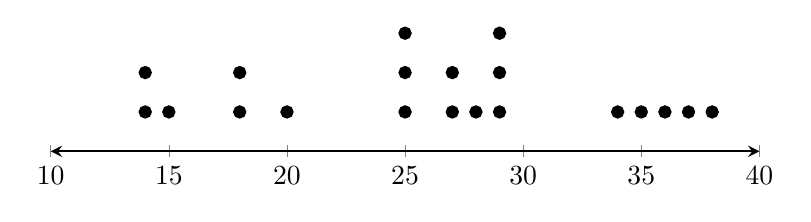
\begin{tikzpicture}
  \begin{axis}[axis lines=center, axis y line=none,
     x=3mm, y=5mm, xtick distance=5,
     axis line style={stealth-stealth, thick},
     xmin=10, xmax=40, ymin=0, ymax=3]
     \addplot [only marks, color=black, thick] coordinates { (14,1) (14,2) (15,1) (18,1) (18,2) (20,1) (25,1) (25,2) (25,3) (27,1) (27,2) (28,1) (29,1) (29,2) (29,3) (34,1) (35,1) (36,1) (37,1) (38,1)  };
  \end{axis}
\end{tikzpicture}



\item

Find the class width of the set: 21, 53, 56, 59, 66, 67, 75, 105 \\[4cm]


\item (2 pts) 
Solve the polynomial equation: $ x^{2} - 2 x - 3 = 0 $. \\[4mm]
\iskey{
    \begin{tabular}{ccl}
        $x^{2} - 2 x - 3$ & $=$ & $(x + 1)(x - 3)$ \\[2mm]
        & $\Rightarrow$ & $x \in \left\{ \mathtt{\text{-1, 3}} \right\}$ \\
    \end{tabular}
}
\item (2 pts) 
Solve the polynomial equation: $ x^{2} + 3 x - 10 = 0 $. \\[4mm]
\iskey{
    \begin{tabular}{ccl}
        $x^{2} + 3 x - 10$ & $=$ & $(x + 5)(x - 2)$ \\[2mm]
        & $\Rightarrow$ & $x \in \left\{ \mathtt{\text{-5, 2}} \right\}$ \\
    \end{tabular}
}


\vspace{3cm}


\item (4 pts) Solve the polynomial equation: $ x^{2} + 6 x - 24 = 0 $. \\[4mm]

\iskey{
    $\displaystyle x^{2} + 6 x = 24 $ \\[4mm]
    $\displaystyle x^{2} + 6 x = 24 $ \\[4mm]
    $\displaystyle x^{2} + 6 x + 9 = 33 $ \\[4mm]
    $\displaystyle \left(x + 3\right)^{2} = 33 $ \\[4mm]
    $\displaystyle \left(x + 3\right)^{2} = 33 $ \\[4mm]
    $\displaystyle x + 3 = \pm \sqrt{33} $ \\[4mm]

    $\displaystyle x \in \left\{ -3 + \sqrt{33}, - \sqrt{33} - 3 \right\}$
}

\end{enumerate}
\end{document}